% Options for packages loaded elsewhere
\PassOptionsToPackage{unicode}{hyperref}
\PassOptionsToPackage{hyphens}{url}
%
\documentclass[
  ignorenonframetext,
]{beamer}
\usepackage{pgfpages}
\setbeamertemplate{caption}[numbered]
\setbeamertemplate{caption label separator}{: }
\setbeamercolor{caption name}{fg=normal text.fg}
\beamertemplatenavigationsymbolsempty
% Prevent slide breaks in the middle of a paragraph
\widowpenalties 1 10000
\raggedbottom
\setbeamertemplate{part page}{
  \centering
  \begin{beamercolorbox}[sep=16pt,center]{part title}
    \usebeamerfont{part title}\insertpart\par
  \end{beamercolorbox}
}
\setbeamertemplate{section page}{
  \centering
  \begin{beamercolorbox}[sep=12pt,center]{part title}
    \usebeamerfont{section title}\insertsection\par
  \end{beamercolorbox}
}
\setbeamertemplate{subsection page}{
  \centering
  \begin{beamercolorbox}[sep=8pt,center]{part title}
    \usebeamerfont{subsection title}\insertsubsection\par
  \end{beamercolorbox}
}
\AtBeginPart{
  \frame{\partpage}
}
\AtBeginSection{
  \ifbibliography
  \else
    \frame{\sectionpage}
  \fi
}
\AtBeginSubsection{
  \frame{\subsectionpage}
}

\usepackage{amsmath,amssymb}
\usepackage{iftex}
\ifPDFTeX
  \usepackage[T1]{fontenc}
  \usepackage[utf8]{inputenc}
  \usepackage{textcomp} % provide euro and other symbols
\else % if luatex or xetex
  \usepackage{unicode-math}
  \defaultfontfeatures{Scale=MatchLowercase}
  \defaultfontfeatures[\rmfamily]{Ligatures=TeX,Scale=1}
\fi
\usepackage{lmodern}
\usetheme[]{Boadilla}
\usecolortheme{rose}
\ifPDFTeX\else  
    % xetex/luatex font selection
\fi
% Use upquote if available, for straight quotes in verbatim environments
\IfFileExists{upquote.sty}{\usepackage{upquote}}{}
\IfFileExists{microtype.sty}{% use microtype if available
  \usepackage[]{microtype}
  \UseMicrotypeSet[protrusion]{basicmath} % disable protrusion for tt fonts
}{}
\makeatletter
\@ifundefined{KOMAClassName}{% if non-KOMA class
  \IfFileExists{parskip.sty}{%
    \usepackage{parskip}
  }{% else
    \setlength{\parindent}{0pt}
    \setlength{\parskip}{6pt plus 2pt minus 1pt}}
}{% if KOMA class
  \KOMAoptions{parskip=half}}
\makeatother
\usepackage{xcolor}
\newif\ifbibliography
\setlength{\emergencystretch}{3em} % prevent overfull lines
\setcounter{secnumdepth}{-\maxdimen} % remove section numbering

\usepackage{color}
\usepackage{fancyvrb}
\newcommand{\VerbBar}{|}
\newcommand{\VERB}{\Verb[commandchars=\\\{\}]}
\DefineVerbatimEnvironment{Highlighting}{Verbatim}{commandchars=\\\{\}}
% Add ',fontsize=\small' for more characters per line
\usepackage{framed}
\definecolor{shadecolor}{RGB}{241,243,245}
\newenvironment{Shaded}{\begin{snugshade}}{\end{snugshade}}
\newcommand{\AlertTok}[1]{\textcolor[rgb]{0.68,0.00,0.00}{#1}}
\newcommand{\AnnotationTok}[1]{\textcolor[rgb]{0.37,0.37,0.37}{#1}}
\newcommand{\AttributeTok}[1]{\textcolor[rgb]{0.40,0.45,0.13}{#1}}
\newcommand{\BaseNTok}[1]{\textcolor[rgb]{0.68,0.00,0.00}{#1}}
\newcommand{\BuiltInTok}[1]{\textcolor[rgb]{0.00,0.23,0.31}{#1}}
\newcommand{\CharTok}[1]{\textcolor[rgb]{0.13,0.47,0.30}{#1}}
\newcommand{\CommentTok}[1]{\textcolor[rgb]{0.37,0.37,0.37}{#1}}
\newcommand{\CommentVarTok}[1]{\textcolor[rgb]{0.37,0.37,0.37}{\textit{#1}}}
\newcommand{\ConstantTok}[1]{\textcolor[rgb]{0.56,0.35,0.01}{#1}}
\newcommand{\ControlFlowTok}[1]{\textcolor[rgb]{0.00,0.23,0.31}{#1}}
\newcommand{\DataTypeTok}[1]{\textcolor[rgb]{0.68,0.00,0.00}{#1}}
\newcommand{\DecValTok}[1]{\textcolor[rgb]{0.68,0.00,0.00}{#1}}
\newcommand{\DocumentationTok}[1]{\textcolor[rgb]{0.37,0.37,0.37}{\textit{#1}}}
\newcommand{\ErrorTok}[1]{\textcolor[rgb]{0.68,0.00,0.00}{#1}}
\newcommand{\ExtensionTok}[1]{\textcolor[rgb]{0.00,0.23,0.31}{#1}}
\newcommand{\FloatTok}[1]{\textcolor[rgb]{0.68,0.00,0.00}{#1}}
\newcommand{\FunctionTok}[1]{\textcolor[rgb]{0.28,0.35,0.67}{#1}}
\newcommand{\ImportTok}[1]{\textcolor[rgb]{0.00,0.46,0.62}{#1}}
\newcommand{\InformationTok}[1]{\textcolor[rgb]{0.37,0.37,0.37}{#1}}
\newcommand{\KeywordTok}[1]{\textcolor[rgb]{0.00,0.23,0.31}{#1}}
\newcommand{\NormalTok}[1]{\textcolor[rgb]{0.00,0.23,0.31}{#1}}
\newcommand{\OperatorTok}[1]{\textcolor[rgb]{0.37,0.37,0.37}{#1}}
\newcommand{\OtherTok}[1]{\textcolor[rgb]{0.00,0.23,0.31}{#1}}
\newcommand{\PreprocessorTok}[1]{\textcolor[rgb]{0.68,0.00,0.00}{#1}}
\newcommand{\RegionMarkerTok}[1]{\textcolor[rgb]{0.00,0.23,0.31}{#1}}
\newcommand{\SpecialCharTok}[1]{\textcolor[rgb]{0.37,0.37,0.37}{#1}}
\newcommand{\SpecialStringTok}[1]{\textcolor[rgb]{0.13,0.47,0.30}{#1}}
\newcommand{\StringTok}[1]{\textcolor[rgb]{0.13,0.47,0.30}{#1}}
\newcommand{\VariableTok}[1]{\textcolor[rgb]{0.07,0.07,0.07}{#1}}
\newcommand{\VerbatimStringTok}[1]{\textcolor[rgb]{0.13,0.47,0.30}{#1}}
\newcommand{\WarningTok}[1]{\textcolor[rgb]{0.37,0.37,0.37}{\textit{#1}}}

\providecommand{\tightlist}{%
  \setlength{\itemsep}{0pt}\setlength{\parskip}{0pt}}\usepackage{longtable,booktabs,array}
\usepackage{calc} % for calculating minipage widths
\usepackage{caption}
% Make caption package work with longtable
\makeatletter
\def\fnum@table{\tablename~\thetable}
\makeatother
\usepackage{graphicx}
\makeatletter
\def\maxwidth{\ifdim\Gin@nat@width>\linewidth\linewidth\else\Gin@nat@width\fi}
\def\maxheight{\ifdim\Gin@nat@height>\textheight\textheight\else\Gin@nat@height\fi}
\makeatother
% Scale images if necessary, so that they will not overflow the page
% margins by default, and it is still possible to overwrite the defaults
% using explicit options in \includegraphics[width, height, ...]{}
\setkeys{Gin}{width=\maxwidth,height=\maxheight,keepaspectratio}
% Set default figure placement to htbp
\makeatletter
\def\fps@figure{htbp}
\makeatother

\makeatletter
\makeatother
\makeatletter
\makeatother
\makeatletter
\@ifpackageloaded{caption}{}{\usepackage{caption}}
\AtBeginDocument{%
\ifdefined\contentsname
  \renewcommand*\contentsname{Table of contents}
\else
  \newcommand\contentsname{Table of contents}
\fi
\ifdefined\listfigurename
  \renewcommand*\listfigurename{List of Figures}
\else
  \newcommand\listfigurename{List of Figures}
\fi
\ifdefined\listtablename
  \renewcommand*\listtablename{List of Tables}
\else
  \newcommand\listtablename{List of Tables}
\fi
\ifdefined\figurename
  \renewcommand*\figurename{Figure}
\else
  \newcommand\figurename{Figure}
\fi
\ifdefined\tablename
  \renewcommand*\tablename{Table}
\else
  \newcommand\tablename{Table}
\fi
}
\@ifpackageloaded{float}{}{\usepackage{float}}
\floatstyle{ruled}
\@ifundefined{c@chapter}{\newfloat{codelisting}{h}{lop}}{\newfloat{codelisting}{h}{lop}[chapter]}
\floatname{codelisting}{Listing}
\newcommand*\listoflistings{\listof{codelisting}{List of Listings}}
\makeatother
\makeatletter
\@ifpackageloaded{caption}{}{\usepackage{caption}}
\@ifpackageloaded{subcaption}{}{\usepackage{subcaption}}
\makeatother
\makeatletter
\@ifpackageloaded{tcolorbox}{}{\usepackage[skins,breakable]{tcolorbox}}
\makeatother
\makeatletter
\@ifundefined{shadecolor}{\definecolor{shadecolor}{rgb}{.97, .97, .97}}
\makeatother
\makeatletter
\makeatother
\makeatletter
\makeatother
\ifLuaTeX
  \usepackage{selnolig}  % disable illegal ligatures
\fi
\IfFileExists{bookmark.sty}{\usepackage{bookmark}}{\usepackage{hyperref}}
\IfFileExists{xurl.sty}{\usepackage{xurl}}{} % add URL line breaks if available
\urlstyle{same} % disable monospaced font for URLs
\hypersetup{
  pdftitle={Recursive Data Structures},
  pdfauthor={Salaar Liaqat},
  hidelinks,
  pdfcreator={LaTeX via pandoc}}

\title{Recursive Data Structures}
\author{Salaar Liaqat}
\date{}
\institute{Data Sciences Institute, UofT}

\begin{document}
\frame{\titlepage}
\ifdefined\Shaded\renewenvironment{Shaded}{\begin{tcolorbox}[borderline west={3pt}{0pt}{shadecolor}, boxrule=0pt, frame hidden, interior hidden, sharp corners, breakable, enhanced]}{\end{tcolorbox}}\fi

\begin{frame}{Outline}
\protect\hypertarget{outline}{}
\begin{itemize}
\item
  Trees
\item
  Anatomy, tree traversal methods
\item
  Binary Search Trees
\item
  Graphs
\item
  Nearest Neighbor Problem
\end{itemize}
\end{frame}

\hypertarget{trees}{%
\section{Trees}\label{trees}}

\begin{frame}{Introduction to Trees}
\protect\hypertarget{introduction-to-trees}{}
\begin{itemize}
\item
  Not all data has a natural linear order. Organization charts and file
  storage systems have a \emph{hierarchical structure}, in which each
  entity is linked to multiple entities below it
\item
  This type of data is represented using a \emph{tree}. A tree is either

  \begin{itemize}
  \item
    Empty
  \item
    Has a \emph{root value} connected to any number of other trees,
    called \emph{subtrees}
  \end{itemize}
\item
  We draw the root at the top of the tree
\end{itemize}
\end{frame}

\begin{frame}{Anatomy of a Tree}
\protect\hypertarget{anatomy-of-a-tree}{}
\begin{columns}[T]
\begin{column}{0.6\textwidth}
\begin{itemize}
\item
  The \emph{size} of a tree is the number of values in the tree
\item
  A \emph{leaf} is a value with no subtrees. The leaves of this tree are
  labeled E, F, G, J, and I
\item
  The \emph{height} of a tree is the longest path from its root to its
  leaves. The height of this tree is 4
\end{itemize}
\end{column}

\begin{column}{0.4\textwidth}
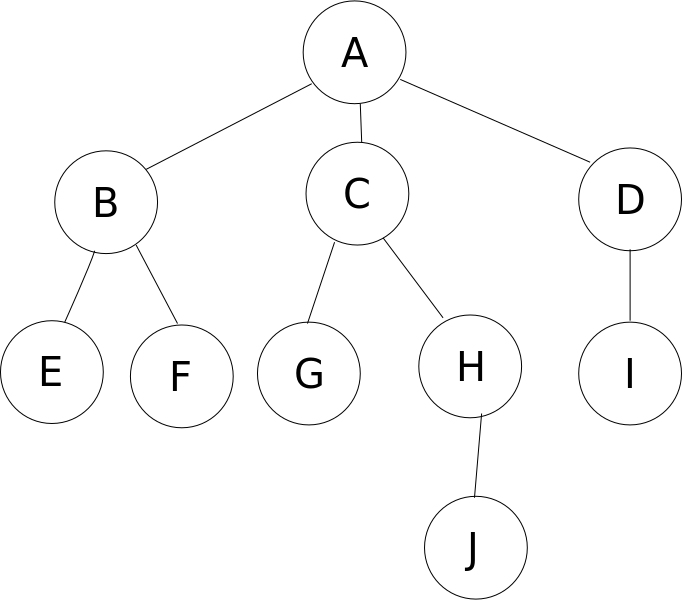
\includegraphics{images/tree.png}
\end{column}
\end{columns}
\end{frame}

\begin{frame}{Anatomy of a Tree}
\protect\hypertarget{anatomy-of-a-tree-1}{}
\begin{columns}[T]
\begin{column}{0.6\textwidth}
\begin{itemize}
\item
  The \emph{children} of a value are all values directly connected
  underneath that value. The children of A are B, C, and D
\item
  The \emph{descendants} of a value are it's children, the children of
  its children, etc. This can be defined recursively
\item
  The \emph{parent} of a value is the value immediately above and
  connected to it. The parent of H is C
\item
  The \emph{ancestors} of a value are its parent, the parent of its
  parent, etc.
\end{itemize}
\end{column}

\begin{column}{0.4\textwidth}
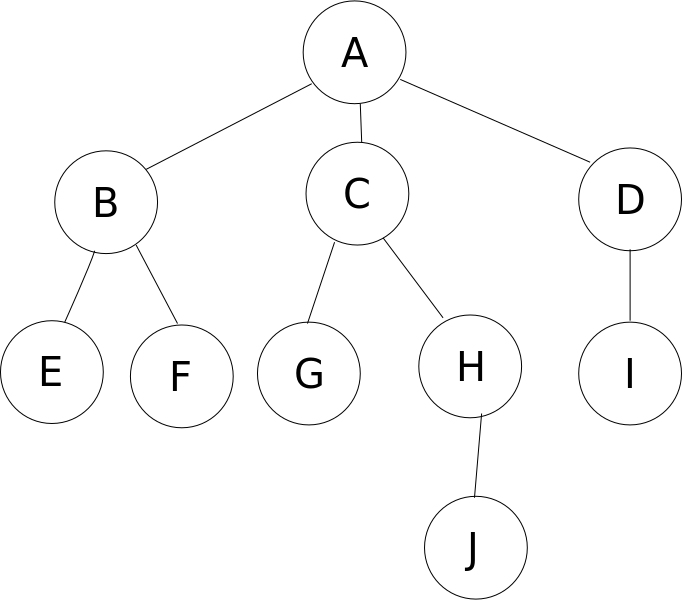
\includegraphics{images/tree.png}
\end{column}
\end{columns}
\end{frame}

\begin{frame}{Tree Traversal Methods}
\protect\hypertarget{tree-traversal-methods}{}
\begin{itemize}
\item
  Linear data structures only have one logical way to traverse them.
  Trees can be traversed in different ways
\item
  We'll look at the following methods of tree traversal and their
  applications

  \begin{itemize}
  \item
    \emph{Depth First Search} (DFS): Inorder, Preorder, and Postorder
    traversal
  \item
    \emph{Breadth First Search} (BFS)
  \end{itemize}
\item
  Note there are other methods not covered
\end{itemize}
\end{frame}

\begin{frame}{DFS: Inorder Traversal}
\protect\hypertarget{dfs-inorder-traversal}{}
\begin{columns}[T]
\begin{column}{0.6\textwidth}
\begin{enumerate}
\item
  Traverse the left subtree
\item
  Visit the root
\item
  Traverse the right subtree
\end{enumerate}

\vspace{1cm}

Result: 4 2 5 1 6 3
\end{column}

\begin{column}{0.4\textwidth}
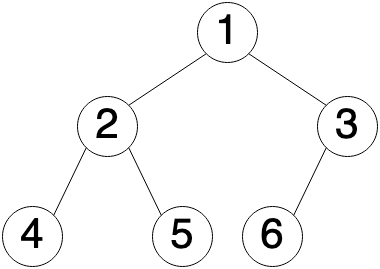
\includegraphics{images/tree-num.png}
\end{column}
\end{columns}
\end{frame}

\begin{frame}[fragile]{DFS: Inorder Traversal Code}
\protect\hypertarget{dfs-inorder-traversal-code}{}
Let's look at the code to do this

\begin{Shaded}
\begin{Highlighting}[]
\KeywordTok{class}\NormalTok{ Node:}
  \CommentTok{"""Tree class}
\CommentTok{  """}
  \KeywordTok{def} \FunctionTok{\_\_init\_\_}\NormalTok{(}\VariableTok{self}\NormalTok{, key):}
    \VariableTok{self}\NormalTok{.left }\OperatorTok{=} \VariableTok{None}
    \VariableTok{self}\NormalTok{.right }\OperatorTok{=} \VariableTok{None}
    \VariableTok{self}\NormalTok{.val }\OperatorTok{=}\NormalTok{ key}
    
\KeywordTok{def}\NormalTok{ print\_inorder(root):}
  \ControlFlowTok{if}\NormalTok{ root:}
\NormalTok{    print\_inorder(root.left)}
    \BuiltInTok{print}\NormalTok{(root.val, end }\OperatorTok{=} \StringTok{" "}\NormalTok{)}
\NormalTok{    print\_inorder(root.right)}
\end{Highlighting}
\end{Shaded}
\end{frame}

\begin{frame}[fragile]{DFS: Inorder Traversal Code}
\protect\hypertarget{dfs-inorder-traversal-code-1}{}
\begin{Shaded}
\begin{Highlighting}[]
\NormalTok{root }\OperatorTok{=}\NormalTok{ Node(}\DecValTok{1}\NormalTok{)}
\NormalTok{root.left }\OperatorTok{=}\NormalTok{ Node(}\DecValTok{2}\NormalTok{)}
\NormalTok{root.right }\OperatorTok{=}\NormalTok{ Node(}\DecValTok{3}\NormalTok{)}
\NormalTok{root.left.left }\OperatorTok{=}\NormalTok{ Node(}\DecValTok{4}\NormalTok{)}
\NormalTok{root.left.right }\OperatorTok{=}\NormalTok{ Node(}\DecValTok{5}\NormalTok{)}
\NormalTok{root.right.left }\OperatorTok{=}\NormalTok{ Node(}\DecValTok{6}\NormalTok{)}
\NormalTok{print\_inorder(root)}
\end{Highlighting}
\end{Shaded}

\begin{verbatim}
4 2 5 1 6 3 
\end{verbatim}

In binary search trees (next section), inorder traversal gives the nodes
in a non-decreasing order.
\end{frame}

\begin{frame}{DFS: Inorder Traversal Complexity}
\protect\hypertarget{dfs-inorder-traversal-complexity}{}
Time complexity

\begin{itemize}
\tightlist
\item
  Each node is visited exactly once. The work done at each node is
  constant. \(O(n)\)
\end{itemize}

Space complexity

\begin{itemize}
\tightlist
\item
  Dependent on the maximum depth of the recursion, which is the height
  of the tree. \(O(h)\)
\end{itemize}
\end{frame}

\begin{frame}{DFS: Preorder Traversal}
\protect\hypertarget{dfs-preorder-traversal}{}
\begin{columns}[T]
\begin{column}{0.6\textwidth}
\begin{enumerate}
\item
  Visit the root
\item
  Traverse the left subtree
\item
  Traverse the right subtree
\end{enumerate}

\vspace{1cm}

Result: 1 2 4 5 3 6

Preorder traversal is used to create a copy of the tree
\end{column}

\begin{column}{0.4\textwidth}
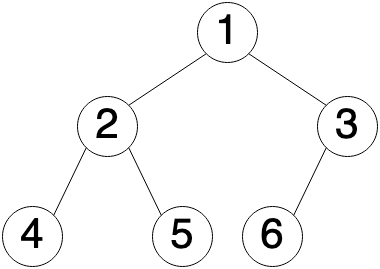
\includegraphics{images/tree-num.png}
\end{column}
\end{columns}
\end{frame}

\begin{frame}{DFS: Postorder Traversal}
\protect\hypertarget{dfs-postorder-traversal}{}
\begin{columns}[T]
\begin{column}{0.6\textwidth}
\begin{enumerate}
\item
  Traverse the left subtree
\item
  Traverse the right subtree
\item
  Visit the root
\end{enumerate}

\vspace{1cm}

Result: 4 5 2 6 3 1

Preorder traversal is used to delete subtrees. (why?)
\end{column}

\begin{column}{0.4\textwidth}
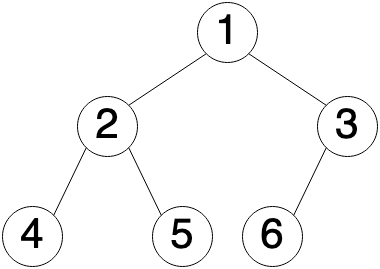
\includegraphics{images/tree-num.png}
\end{column}
\end{columns}
\end{frame}

\begin{frame}{BFS}
\protect\hypertarget{bfs}{}
\begin{columns}[T]
\begin{column}{0.6\textwidth}
BFS (or Level Order Traversal) traverses nodes present in the same level
before traversing the next level

\begin{enumerate}
\tightlist
\item
  For each node
\end{enumerate}

\begin{itemize}
\item
  The node is visited
\item
  The child nodes are enqueued in a FIFO queue
\end{itemize}

\begin{enumerate}
\setcounter{enumi}{1}
\item
  First node is dequeued
\item
  Child nodes are enqueued
\item
  Repeat until the queue is empty
\end{enumerate}

Result: 1 2 3 4 5 6
\end{column}

\begin{column}{0.4\textwidth}
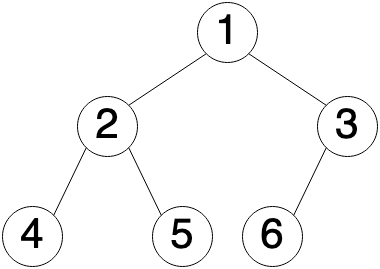
\includegraphics{images/tree-num.png}
\end{column}
\end{columns}
\end{frame}

\hypertarget{binary-search-trees}{%
\section{Binary Search Trees}\label{binary-search-trees}}

\begin{frame}{BST Definitions}
\protect\hypertarget{bst-definitions}{}
\begin{itemize}
\item
  You can think of a BST as a sorted tree
\item
  A \emph{binary tree} is a tree in which every item has at most two
  subtrees

  \begin{itemize}
  \tightlist
  \item
    The tree used in illustrating DFS and BFS methods is a binary tree
  \end{itemize}
\item
  A binary tree is a \emph{binary search tree property} if its value is
  greater than or equal to all items in the left subtree
\item
  A binary tree is a \emph{binary search tree} if every item in the tree
  satisfies the binary search tree property
\end{itemize}
\end{frame}

\begin{frame}{BST Efficiency}
\protect\hypertarget{bst-efficiency}{}
\begin{columns}[T]
\begin{column}{0.7\textwidth}
\begin{itemize}
\item
  Consider the BST on the right. Verify that it is a BST.
\item
  The worst-case run time is \(O(h)\), \(h\) being the height of the
  tree

  \begin{itemize}
  \tightlist
  \item
    So the tree on the right is \(O(n)\)
  \end{itemize}
\item
  A tree of height \(h\) can have at most \(2^h - 1\) nodes. So we need
  at least log\(n\) height to store all of them.

  \begin{itemize}
  \tightlist
  \item
    So if the tree was balanced, then it would be \(O(\text{log}n)\)
  \end{itemize}
\end{itemize}
\end{column}

\begin{column}{0.3\textwidth}
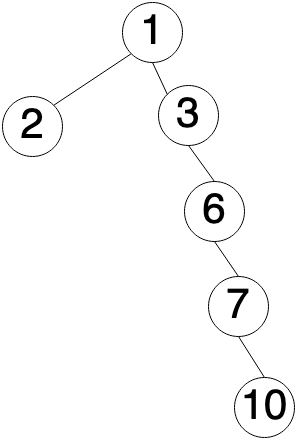
\includegraphics{images/tree-unbal.png}
\end{column}
\end{columns}
\end{frame}

\begin{frame}{BST Efficiency}
\protect\hypertarget{bst-efficiency-1}{}
\begin{itemize}
\item
  Convince yourself that for a balanced BST the search, insert, and
  delete Big-O is all \(O(\text{log}n)\)
\item
  Ensuring that a tree is balanced is important

  \begin{itemize}
  \item
    Red-Black trees (not covered) are trees that balance themselves
  \item
    You may also be interested in B-trees, which are used in databases
  \end{itemize}
\end{itemize}
\end{frame}

\begin{frame}{Live Coding}
\protect\hypertarget{live-coding}{}
Given a BST, insert a new node in this BST.

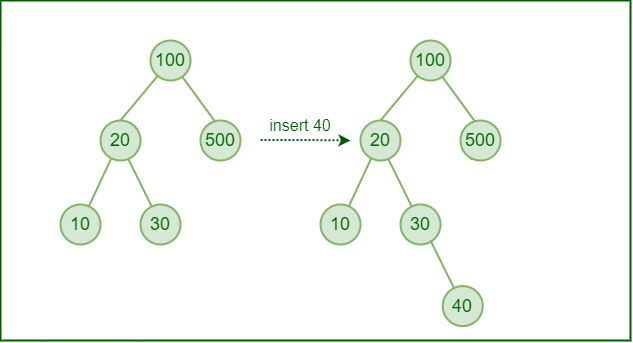
\includegraphics[width=4.80208in,height=\textheight]{images/insertion.png}
\end{frame}

\hypertarget{graphs}{%
\section{Graphs}\label{graphs}}

\begin{frame}{Introduction}
\protect\hypertarget{introduction}{}
\begin{itemize}
\item
  We looked at lists and trees, which represent linear and hierarchical
  relationships respectively

  \begin{itemize}
  \item
    But many relationships are neither
  \item
    Friend networks, internet connections, flight connections
  \end{itemize}
\item
  Graphs consist of two parts, \emph{nodes} and \emph{edges}

  \begin{itemize}
  \tightlist
  \item
    A node connected to another is a \emph{neighbor} \vspace{1cm}
  \end{itemize}
\end{itemize}

\begin{figure}

{\centering 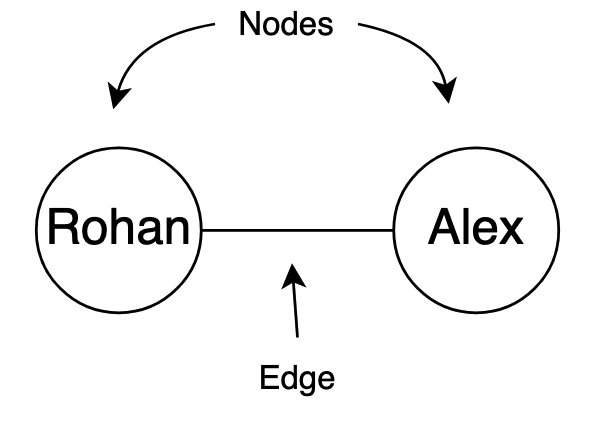
\includegraphics[width=1.625in,height=\textheight]{images/graph-anat.png}

}

\end{figure}
\end{frame}

\begin{frame}{Types of Graphs}
\protect\hypertarget{types-of-graphs}{}
\begin{columns}[T]
\begin{column}{0.6\textwidth}
There are directed and undirected graphs to represent different
situations

\begin{itemize}
\item
  Friendships: undirected
\item
  Twitter followers: directed
\item
  Who owes who money: directed
\item
  Note that trees are special cases of directed graphs
\end{itemize}

Graphs can also be weighted, to differentiate strengths between nodes

There are two questions we ask about graphs: Is there a path from node A
to B? What is the shortest path from node A to B? BFS answers both!
\end{column}

\begin{column}{0.4\textwidth}
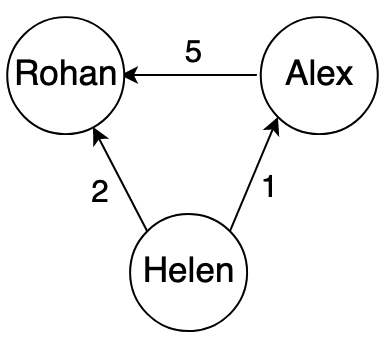
\includegraphics{images/graph-weight.png}
\end{column}
\end{columns}
\end{frame}

\begin{frame}{BFS of Graphs}
\protect\hypertarget{bfs-of-graphs}{}
\begin{itemize}
\item
  \emph{Breadth First Search} (BFS) searches graph for a node that meets
  a set of criteria. It starts at the root of the graph and visits all
  nodes at the current depth level before moving on to the nodes at the
  next depth level

  \begin{itemize}
  \tightlist
  \item
    If there are multiple nodes meeting the criteria, then BFS will also
    find the nearest node!
  \end{itemize}
\item
  The issue is that graphs contain \emph{cycles}, so we may visit the
  same node more than once

  \begin{itemize}
  \tightlist
  \item
    Let's split edges into visited and not visited
  \end{itemize}
\item
  We use a list to keep track of visited nodes
\item
  All the adjacent unvisited nodes of the current level are pushed into
  the queue and the nodes of the current level are marked visited and
  popped from the queue
\item
  Is BFS a recursive or iterative graph search method?
\end{itemize}
\end{frame}

\begin{frame}{BFS Example}
\protect\hypertarget{bfs-example}{}
\begin{columns}[T]
\begin{column}{0.6\textwidth}
\begin{itemize}
\item
  Let's traverse a graph with BFS starting at node ``1''
\item
  Visited list and queue start as empty \vspace{1cm}
\end{itemize}

Visited: {[} , , , , {]}

Queue: {[} , , , , {]}
\end{column}

\begin{column}{0.4\textwidth}
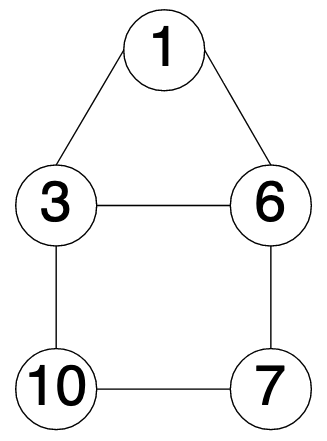
\includegraphics{images/graph-bfs.png}
\end{column}
\end{columns}
\end{frame}

\begin{frame}{BFS Example}
\protect\hypertarget{bfs-example-1}{}
\begin{columns}[T]
\begin{column}{0.6\textwidth}
\begin{itemize}
\tightlist
\item
  We're at node 1, so we push it onto the visited list and push it onto
  the queue \vspace{1cm}
\end{itemize}

Visited: {[}1, , , , {]}

Queue: {[}1, , , , {]}
\end{column}

\begin{column}{0.4\textwidth}
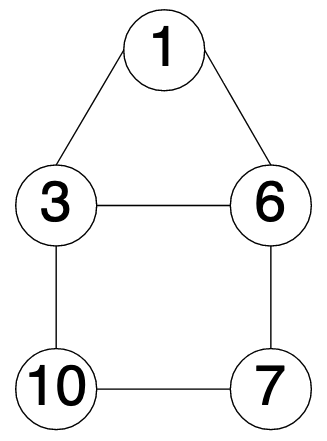
\includegraphics{images/graph-bfs.png}
\end{column}
\end{columns}
\end{frame}

\begin{frame}{BFS Example}
\protect\hypertarget{bfs-example-2}{}
\begin{columns}[T]
\begin{column}{0.6\textwidth}
\begin{itemize}
\item
  Now we visited 1, so it is dequeued.
\item
  At the first level away from node 1, there is 3 and 6.
\item
  We visit 3 and 6, but we have not visited any of it's neighbors (other
  than 1), so 3 and 6 are enqueued. \vspace{1cm}
\end{itemize}

Visited: {[}1, 3, 6, , {]}

Queue: {[}3, 6, , , {]}
\end{column}

\begin{column}{0.4\textwidth}
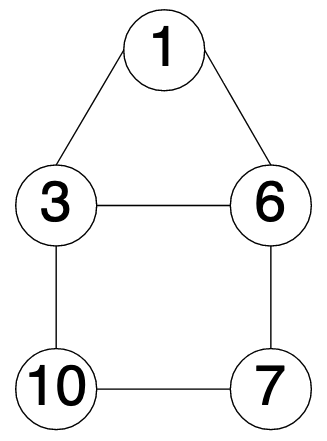
\includegraphics{images/graph-bfs.png}
\end{column}
\end{columns}
\end{frame}

\begin{frame}{BFS Example}
\protect\hypertarget{bfs-example-3}{}
\begin{columns}[T]
\begin{column}{0.6\textwidth}
\begin{itemize}
\item
  Visit the neighbors of node 3, so we dequeue it
\item
  But we need to enqueue 10, because we haven't visited its neighbors
  \vspace{1cm}
\end{itemize}

Visited: {[}1, 3, 6, 10, {]}

Queue: {[}6, 10, , {]}
\end{column}

\begin{column}{0.4\textwidth}
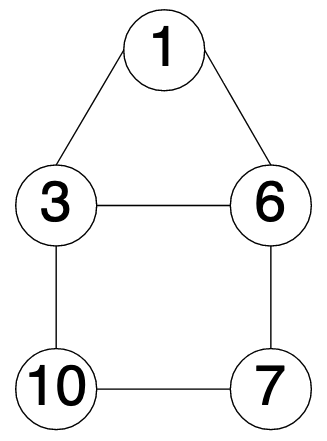
\includegraphics{images/graph-bfs.png}
\end{column}
\end{columns}
\end{frame}

\begin{frame}{BFS Example}
\protect\hypertarget{bfs-example-4}{}
\begin{columns}[T]
\begin{column}{0.6\textwidth}
\begin{itemize}
\item
  Visit the neighbors of node 6, which is just 7, so we dequeue it
\item
  But we need to enqueue 7 \vspace{1cm}
\end{itemize}

Visited: {[}1, 3, 6, 10, 7{]}

Queue: {[}10, 7, , {]}
\end{column}

\begin{column}{0.4\textwidth}
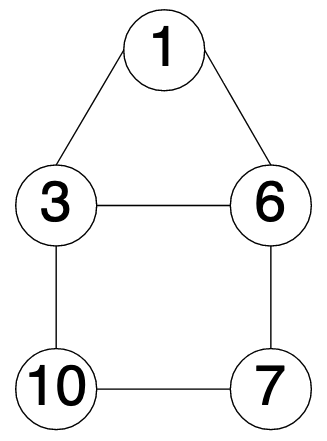
\includegraphics{images/graph-bfs.png}
\end{column}
\end{columns}
\end{frame}

\begin{frame}{BFS Example}
\protect\hypertarget{bfs-example-5}{}
\begin{columns}[T]
\begin{column}{0.6\textwidth}
\begin{itemize}
\item
  Visit the neighbors of node 10, and dequeue 10
\item
  But we already visited those nodes, so the visited list does not
  change \vspace{1cm}
\end{itemize}

Visited: {[}1, 3, 6, 10, 7{]}

Queue: {[}7, , , , {]}
\end{column}

\begin{column}{0.4\textwidth}
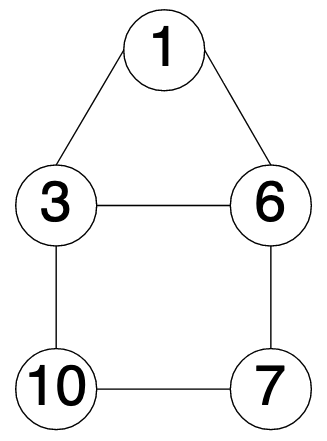
\includegraphics{images/graph-bfs.png}
\end{column}
\end{columns}
\end{frame}

\begin{frame}{BFS Example}
\protect\hypertarget{bfs-example-6}{}
\begin{columns}[T]
\begin{column}{0.6\textwidth}
\begin{itemize}
\item
  Visit neighbors of 7, which are also all visited
\item
  The queue is empty, so the algorithm ends \vspace{1cm}
\end{itemize}

Visited: {[}1, 3, 6, 10, 7{]}

Queue: {[} , , , , {]}
\end{column}

\begin{column}{0.4\textwidth}
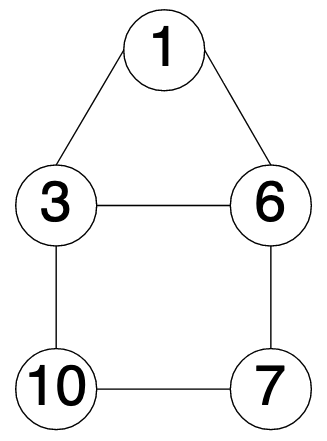
\includegraphics{images/graph-bfs.png}
\end{column}
\end{columns}
\end{frame}

\begin{frame}{Time and Space Complexity of BFS}
\protect\hypertarget{time-and-space-complexity-of-bfs}{}
\begin{itemize}
\item
  Each edge and each node must be visited once, so the time complexity
  is \(O(n + e)\)
\item
  Since we need to store each node of the graph by the end of the
  algorithm, the space complexity is \(O(n)\)
\end{itemize}
\end{frame}

\begin{frame}[fragile]{Implementing Graphs and BFS}
\protect\hypertarget{implementing-graphs-and-bfs}{}
We can represent graphs using the \emph{adjacency list} representation

\begin{itemize}
\tightlist
\item
  Other options include adjacency matrix or using a Python library
\end{itemize}

\begin{Shaded}
\begin{Highlighting}[]
\ImportTok{from}\NormalTok{ collections }\ImportTok{import}\NormalTok{ deque}

\KeywordTok{class}\NormalTok{ Graph:}
  \KeywordTok{def} \FunctionTok{\_\_init\_\_}\NormalTok{(}\VariableTok{self}\NormalTok{):}
    \VariableTok{self}\NormalTok{.graph }\OperatorTok{=}\NormalTok{ \{\}}

  \KeywordTok{def}\NormalTok{ add\_edge(}\VariableTok{self}\NormalTok{, vertex, neighbors):}
    \VariableTok{self}\NormalTok{.graph[vertex] }\OperatorTok{=}\NormalTok{ neighbors}
\end{Highlighting}
\end{Shaded}
\end{frame}

\begin{frame}[fragile]{Implementing Graphs and BFS}
\protect\hypertarget{implementing-graphs-and-bfs-1}{}
\begin{Shaded}
\begin{Highlighting}[]
\KeywordTok{def}\NormalTok{ bfs(graph, start):}
\NormalTok{  visited }\OperatorTok{=} \BuiltInTok{set}\NormalTok{()}
\NormalTok{  queue }\OperatorTok{=}\NormalTok{ deque([start])}

  \ControlFlowTok{while}\NormalTok{ queue:}
\NormalTok{    current\_vertex }\OperatorTok{=}\NormalTok{ queue.popleft()}

    \ControlFlowTok{if}\NormalTok{ current\_vertex }\KeywordTok{not} \KeywordTok{in}\NormalTok{ visited:}
      \CommentTok{\# Process the current vertex}
      \BuiltInTok{print}\NormalTok{(current\_vertex, end}\OperatorTok{=}\StringTok{\textquotesingle{} \textquotesingle{}}\NormalTok{)}
\NormalTok{      visited.add(current\_vertex)}

      \CommentTok{\# Enqueue unvisited neighbors}
      \ControlFlowTok{for}\NormalTok{ neighbor }\KeywordTok{in}\NormalTok{ graph.graph.get(current\_vertex, []):}
        \ControlFlowTok{if}\NormalTok{ neighbor }\KeywordTok{not} \KeywordTok{in}\NormalTok{ visited:}
\NormalTok{          queue.append(neighbor)}
\end{Highlighting}
\end{Shaded}
\end{frame}

\begin{frame}[fragile]{Implementing Graphs and BFS}
\protect\hypertarget{implementing-graphs-and-bfs-2}{}
\begin{Shaded}
\begin{Highlighting}[]
\CommentTok{\# Represent graph from above}
\NormalTok{ex\_graph }\OperatorTok{=}\NormalTok{ Graph()}
\NormalTok{ex\_graph.add\_edge(}\DecValTok{1}\NormalTok{, [}\DecValTok{3}\NormalTok{, }\DecValTok{6}\NormalTok{])}
\NormalTok{ex\_graph.add\_edge(}\DecValTok{3}\NormalTok{, [}\DecValTok{10}\NormalTok{, }\DecValTok{6}\NormalTok{])}
\NormalTok{ex\_graph.add\_edge(}\DecValTok{6}\NormalTok{, [}\DecValTok{3}\NormalTok{, }\DecValTok{7}\NormalTok{])}
\NormalTok{ex\_graph.add\_edge(}\DecValTok{10}\NormalTok{, [}\DecValTok{3}\NormalTok{, }\DecValTok{7}\NormalTok{])}
\NormalTok{ex\_graph.add\_edge(}\DecValTok{7}\NormalTok{, [}\DecValTok{10}\NormalTok{, }\DecValTok{6}\NormalTok{])}

\CommentTok{\# Perform BFS starting from vertex 1}
\NormalTok{bfs(ex\_graph, }\DecValTok{1}\NormalTok{)}
\end{Highlighting}
\end{Shaded}

\begin{verbatim}
1 3 6 10 7 
\end{verbatim}
\end{frame}

\begin{frame}[fragile]{Recursive Graph Search: Preorder Traversal}
\protect\hypertarget{recursive-graph-search-preorder-traversal}{}
\begin{itemize}
\tightlist
\item
  Using the same \texttt{Graph} class, let's implement preorder
  traversal
\end{itemize}

\begin{Shaded}
\begin{Highlighting}[]
\KeywordTok{def}\NormalTok{ recursive\_preorder\_traversal(graph, start, visited}\OperatorTok{=}\VariableTok{None}\NormalTok{):}
  \ControlFlowTok{if}\NormalTok{ visited }\KeywordTok{is} \VariableTok{None}\NormalTok{:}
\NormalTok{    visited }\OperatorTok{=} \BuiltInTok{set}\NormalTok{()}

  \CommentTok{\# Process the current vertex}
  \BuiltInTok{print}\NormalTok{(start, end}\OperatorTok{=}\StringTok{\textquotesingle{} \textquotesingle{}}\NormalTok{)}
\NormalTok{  visited.add(start)}

    \CommentTok{\# Recursive traversal of neighbors}
  \ControlFlowTok{for}\NormalTok{ neighbor }\KeywordTok{in}\NormalTok{ graph.graph.get(start, []):}
    \ControlFlowTok{if}\NormalTok{ neighbor }\KeywordTok{not} \KeywordTok{in}\NormalTok{ visited:}
\NormalTok{      recursive\_preorder\_traversal(graph, neighbor, visited)}
\end{Highlighting}
\end{Shaded}
\end{frame}

\begin{frame}[fragile]{Recursive Graph Search: Preorder Traversal}
\protect\hypertarget{recursive-graph-search-preorder-traversal-1}{}
\begin{Shaded}
\begin{Highlighting}[]
\NormalTok{bfs(ex\_graph, }\DecValTok{1}\NormalTok{)}
\end{Highlighting}
\end{Shaded}

\begin{verbatim}
1 3 6 10 7 
\end{verbatim}
\end{frame}

\hypertarget{nearest-neighour-problem}{%
\section{Nearest Neighour Problem}\label{nearest-neighour-problem}}

\begin{frame}{Nearest Neighbour Problem}
\protect\hypertarget{nearest-neighbour-problem}{}
\begin{itemize}
\item
  As you may have encountered already, machine learning and statistical
  methods often depend on finding the nearest neighbor to a data point

  \begin{itemize}
  \tightlist
  \item
    K-nearest neighbors regression, propensity score matching
  \end{itemize}
\item
  In a \(k\) dimensional space, if we conduct a linear search for
  points, the running time will be \(O(kn)\) for \(n\) data points.
\item
  Can we do better?
\end{itemize}
\end{frame}

\begin{frame}{k-d Trees}
\protect\hypertarget{k-d-trees}{}
\begin{itemize}
\item
  k-d trees is short for k dimensional tree (notation is a bit
  unfortunate, different K than KNN)

  \begin{itemize}
  \tightlist
  \item
    It is useful for multidimensional searches
  \end{itemize}
\item
  Let's discuss the properties of k-d trees and why they work
\item
  Binary tree where each node represents an axis-aligned hyperrectangle
  in the k-dimensional space

  \begin{itemize}
  \tightlist
  \item
    hyperrectangle: rectangle in higher dimensions
  \end{itemize}
\item
  Nodes in the left subtree have coordinates less than the splitting
  dimension of the current node, while nodes in the right subtree have
  coordinates greater than the splitting dimension.
\item
  At each level of the tree, a specific dimension is chosen to split the
  data. The choice of dimension alternates as we traverse down the tree.
\item
  Each leaf represents a single point in the k-dimensional space
\end{itemize}
\end{frame}

\begin{frame}{k-d Trees Animation}
\protect\hypertarget{k-d-trees-animation}{}
\url{https://commons.wikimedia.org/wiki/File:KDTree-animation.gif}
\end{frame}

\begin{frame}{Applications and Issues}
\protect\hypertarget{applications-and-issues}{}
\begin{itemize}
\item
  Notice k-d trees can also find values within a certain range very
  quickly, not just a specific point
\item
  GIS (geographic information systems) queries
\item
  KNN algorithm
\item
  Computer graphics, such as ray tracing to facilitate efficient space
  partitioning
\item
  Issues occur in high-dimensional spaces and trees can become
  imbalanced
\end{itemize}
\end{frame}

\hypertarget{recommended-problems-and-references}{%
\section{Recommended Problems and
References}\label{recommended-problems-and-references}}

\begin{frame}{Recommended Readings}
\protect\hypertarget{recommended-readings}{}
\begin{itemize}
\item
  Bhargava: Chapter 6
\item
  Bhargava: Chapter 11, pages 203 to 206 about Trees
\end{itemize}
\end{frame}

\begin{frame}{Recommended Problems}
\protect\hypertarget{recommended-problems}{}
\begin{itemize}
\item
  Cormen: Chapter 10 exercises

  \begin{itemize}
  \tightlist
  \item
    10.3-1, 10.3-2, 10.3-3
  \end{itemize}
\item
  Bhargava: Chapter 6 exercises

  \begin{itemize}
  \tightlist
  \item
    6.1 to 6.5
  \end{itemize}
\end{itemize}
\end{frame}

\begin{frame}[fragile]{Recommended Problems}
\protect\hypertarget{recommended-problems-1}{}
\begin{itemize}
\item
  Implement preorder, postorder, and level order traversal. Determine
  the time and space complexity in each case
\item
  Implement a function that find an element in a BST and deletes it. The
  descendants of the deleted node are given to the deleted node's
  parent.
\item
  Using the \texttt{graph} class from the slides, implement BST search
  such that it stops and tell you the distance the node is from the
  starting point.

  \begin{itemize}
  \item
    For instance, if we searched for 7 in the graph given in the slides,
    it would return \texttt{"Found!\ Distance\ 2"}.
  \item
    If we searched for 100 in the graph, it would return
    \texttt{"Not\ found!"}
  \end{itemize}
\item
  Implement postorder graph traversal using the \texttt{graph} class
  from the slides.
\item
  Implement a function using recursion to find the sum heterogeneous
  nested lists such as {[}{[}1, {[}2{]}{]}, {[}{[}{[}3{]}{]}{]}, 4,
  {[}{[}5, 6{]}, {[}{[}{[}7{]}{]}{]}{]}{]}.
\end{itemize}
\end{frame}

\begin{frame}{References}
\protect\hypertarget{references}{}
\begin{itemize}
\item
  Bhargava, A. Y. (2016). \emph{Grokking algorithms: An illustrated
  guide for programmers and other curious people.} Manning. Chapter 6,
  10, 11.
\item
  Cormen, T. H. (Ed.). (2009). \emph{Introduction to algorithms} (3rd
  ed). MIT Press. Chapter 12 and 20.
\item
  Horton, D., \& Liu, D. (2023, November 19). \emph{CSC148 Lecture
  Notes}.
  https://www.teach.cs.toronto.edu/\textasciitilde csc148h/winter/notes/
\end{itemize}
\end{frame}



\end{document}
